\documentclass{article}

\usepackage[LGR, T1]{fontenc}
\usepackage[utf8]{inputenc}
\usepackage[greek,english]{babel}
\usepackage{alphabeta}
\usepackage{graphicx}
\graphicspath{{./}}


\author{Στεφανίδης Ιωάννης}
\title{Δίκτυα Υπολογιστών ΙΙ}
\date{ΑΕΜ: 9587}


\begin{document}

\maketitle

\section{Σχόλια και Παρατηρήσεις}

Η αλήθεια είναι ότι ζητήσατε τον πιο απλό κώδικα που να παίρνει από την Ιθάκη
τα δεδομένα που χρειαζόμαστε για να κάνουμε την εργασία. Εγώ όμως προσπάθησα να
φτιάξω ένα είδους API (Application Programming Interface) για την Ιθάκη που
έχει κλάσεις για κάθε πληροφορία που μπορείς να ζητήσεις. Για παράδειγμα
μπορείτε να δείτε την κλάση \texttt{VehiclePacket} όπου δεν μας ενδιαφέρει να
δούμε την απάντηση από την Ιθάκη αλλά πρέπει να κάνουμε parse το String του
πακέτου σύμφωνα με το OBD-II για να πάρουμε τις πληροφορίες του οχήματος.

Στο \texttt{IHAKI\_API} θα βρείτε τις συναρτήσεις \texttt{getPacket,
getImage, getSound, getTelemetry} και \texttt{getVehiclePacket} όλες αυτές
επιστρέφουν την custom class που έχει φτιαχτεί για το κάθε κομμάτι και
όχι την απάντηση της Ιθάκης.

\section{Πρωτόκολλο Αυτοδύναμων Πακέτων Χρήστη - UDP}

Το Πρωτόκολλο Αυτοδύναμων Πακέτων Χρήστη (User Datagram Protocol)\cite{udpwebsite}
παρέχει το βασικό μηχανισμό που χρησιμοποιούν τα προγράμματα εφαρμογών για να
στέλνουν αυτοδύναμα πακέτα σε άλλα προγράμματα εφαρμογών. Το UDP παρέχει θύρες
πρωτοκόλλων που χρησιμεύουν στη διάκριση μεταξύ των προγραμμάτων τα οποία
εκτελούνται σε μια μηχανή. Με άλλα λόγια, κάθε μήνυμα UDP περιλαμβάνει, εκτός
από τα δεδομένα, έναν αριθμό θύρας προορισμού και έναν αριθμό θύρας προέλευσης,
γεγονός που δίνει τη δυνατότητα στο λογισμικό UDP του προορισμού να παραδώσει
το μήνυμα στο σωστό παραλήπτη, και επίσης επιτρέπει στον παραλήπτη να στείλει
μια απάντηση.

Το UDP χρησιμοποιεί το Πρωτόκολλο Internet για να μεταφέρει ένα μήνυμα από μια
μηχανή σε μια άλλη, και παρέχει την ίδια μη αξιόπιστη, ασυνδεσμική παράδοση
αυτοδύνα­μων πακέτων όπως και το ΙΡ.
\begin{itemize}
  \item Δε χρησιμοποιεί σήματα επιβεβαίωσης για να σιγουρευτεί ότι τα μηνύματα
 έφτασαν στον προορισμό τους,
  \item Δεν ταξινομεί τα εισερχόμενα μηνύματα, και
  \item Δεν παρέχει ανατροφοδότηση για να ελέγξει το ρυθμό ροής των πληροφοριών
 μεταξύ των μηχα­νημάτων.
\end{itemize}

Άρα, τα μηνύματα UDP μπορεί να χαθούν, να αναπαραχθούν, ή να φτάσουν στον
προορισμό τους εκτός σειράς. Επιπλέον, τα πακέτα μπορεί να φτάνουν πολύ γρήγορα
και ο δέκτης να μην προλαβαίνει να τα επεξεργαστεί. Συνοψίζοντας μπορούμε να
πούμε τα εξής:

Το Πρωτόκολλο Αυτοδύναμων Πακέτων Χρήστη (UDP) παρέχει μια αναξιόπιστη,
ασυνδεσμική υπηρεσία παράδοσης, χρησιμοποιώντας το ΙΡ για τη μεταφορά μηνυμάτων
μεταξύ μηχανών. Χρησιμοποιεί το ΙΡ για να μεταφέρει μηνύματα, δίνει όμως και τη
δυνατότητα διάκρισης μεταξύ πολλαπλών προορισμών σε ένα δεδομένο υπολογιστή
υπηρεσίας.

Επίσης ένα πρόγραμμα εφαρμογής που χρησιμοποιεί UDP είναι αποκλειστικά υπεύθυνο για το
χειρισμό του προβλήματος της αξιοπιστίας και όσων αυτό συνεπάγεται, όπως η
απώλεια μηνύματος, η αναπαραγωγή μηνύματος, η καθυστέρηση και η παράδοση εκτός
σειράς.

\section{VPN}

Δεν χρησιμοποίησα port forwarding ούτε έκανα κάποια ρύθμιση στο router μου καθώς
δεν έχω πρόσβαση σε αυτό λόγω του ISP μου (SkyTelecom).
Συνδέθηκα όμως με το VPN που μας δίνει το ΑΠΘ και στην εικόνα φαίνεται αυτή η
σύνδεση.\\

\centering
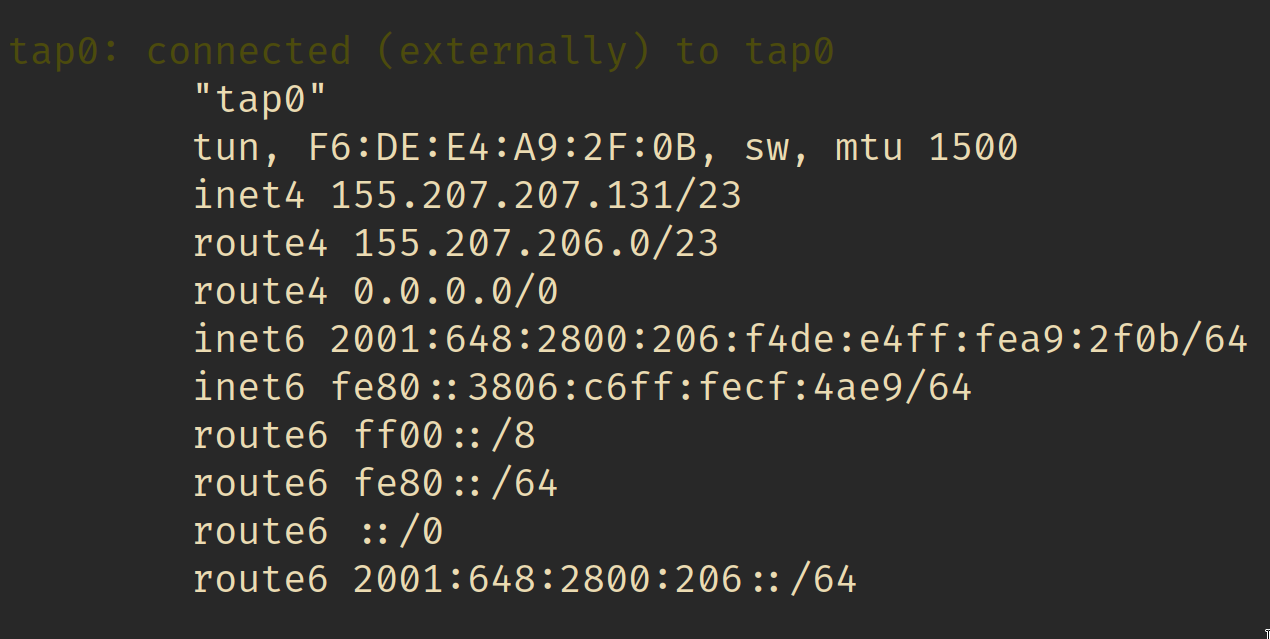
\includegraphics[width=0.8\textwidth]{vpn}



\begin{thebibliography}{9}

\bibitem{udpwebsite}
Πρωτόκολλο Αυτοδύναμων Πακέτων Χρήστη - UDP
\\\texttt{http://conta.uom.gr/conta/ekpaideysh/metaptyxiaka/technologies\_diktywn
/ergasies/2005/html/IP/12/12.1.htm}
\end{thebibliography}

\end{document}
